\section{Phase 5 - Refining the Initial Baseline using Reinforcement Learning}

As explained earlier in Section~\ref{sec:background}, the emotion baseline of a user is not something fixed. It can change over time depending on the person's mood, situation, and other conditions. Because of that, our system needs a way to update this baseline from time to time. But we also want to do this with minimal inputs from the user.

To solve this problem, we are using a Reinforcement Learning (RL) framework. More specifically, we use Q-learning to refine the emotional baseline in the arousal-valence plane. This method helps the system to learn how to adjust the baseline gradually, based on the feedback it gets and how well it performs. It also works with very little direct input from the user.

Sometimes, the user gives direct feedback using a simple emoji-based system. These emojis help the system understand how the user is feeling in a lightweight and non-intrusive way. The overall idea of this stage is shown in Figure~\ref{fig:phase5}.

Prior to examining the structure and functioning of the RL model, the operation of the emoji feedback mechanism is first considered.

\begin{figure*}[h]
    \centering
    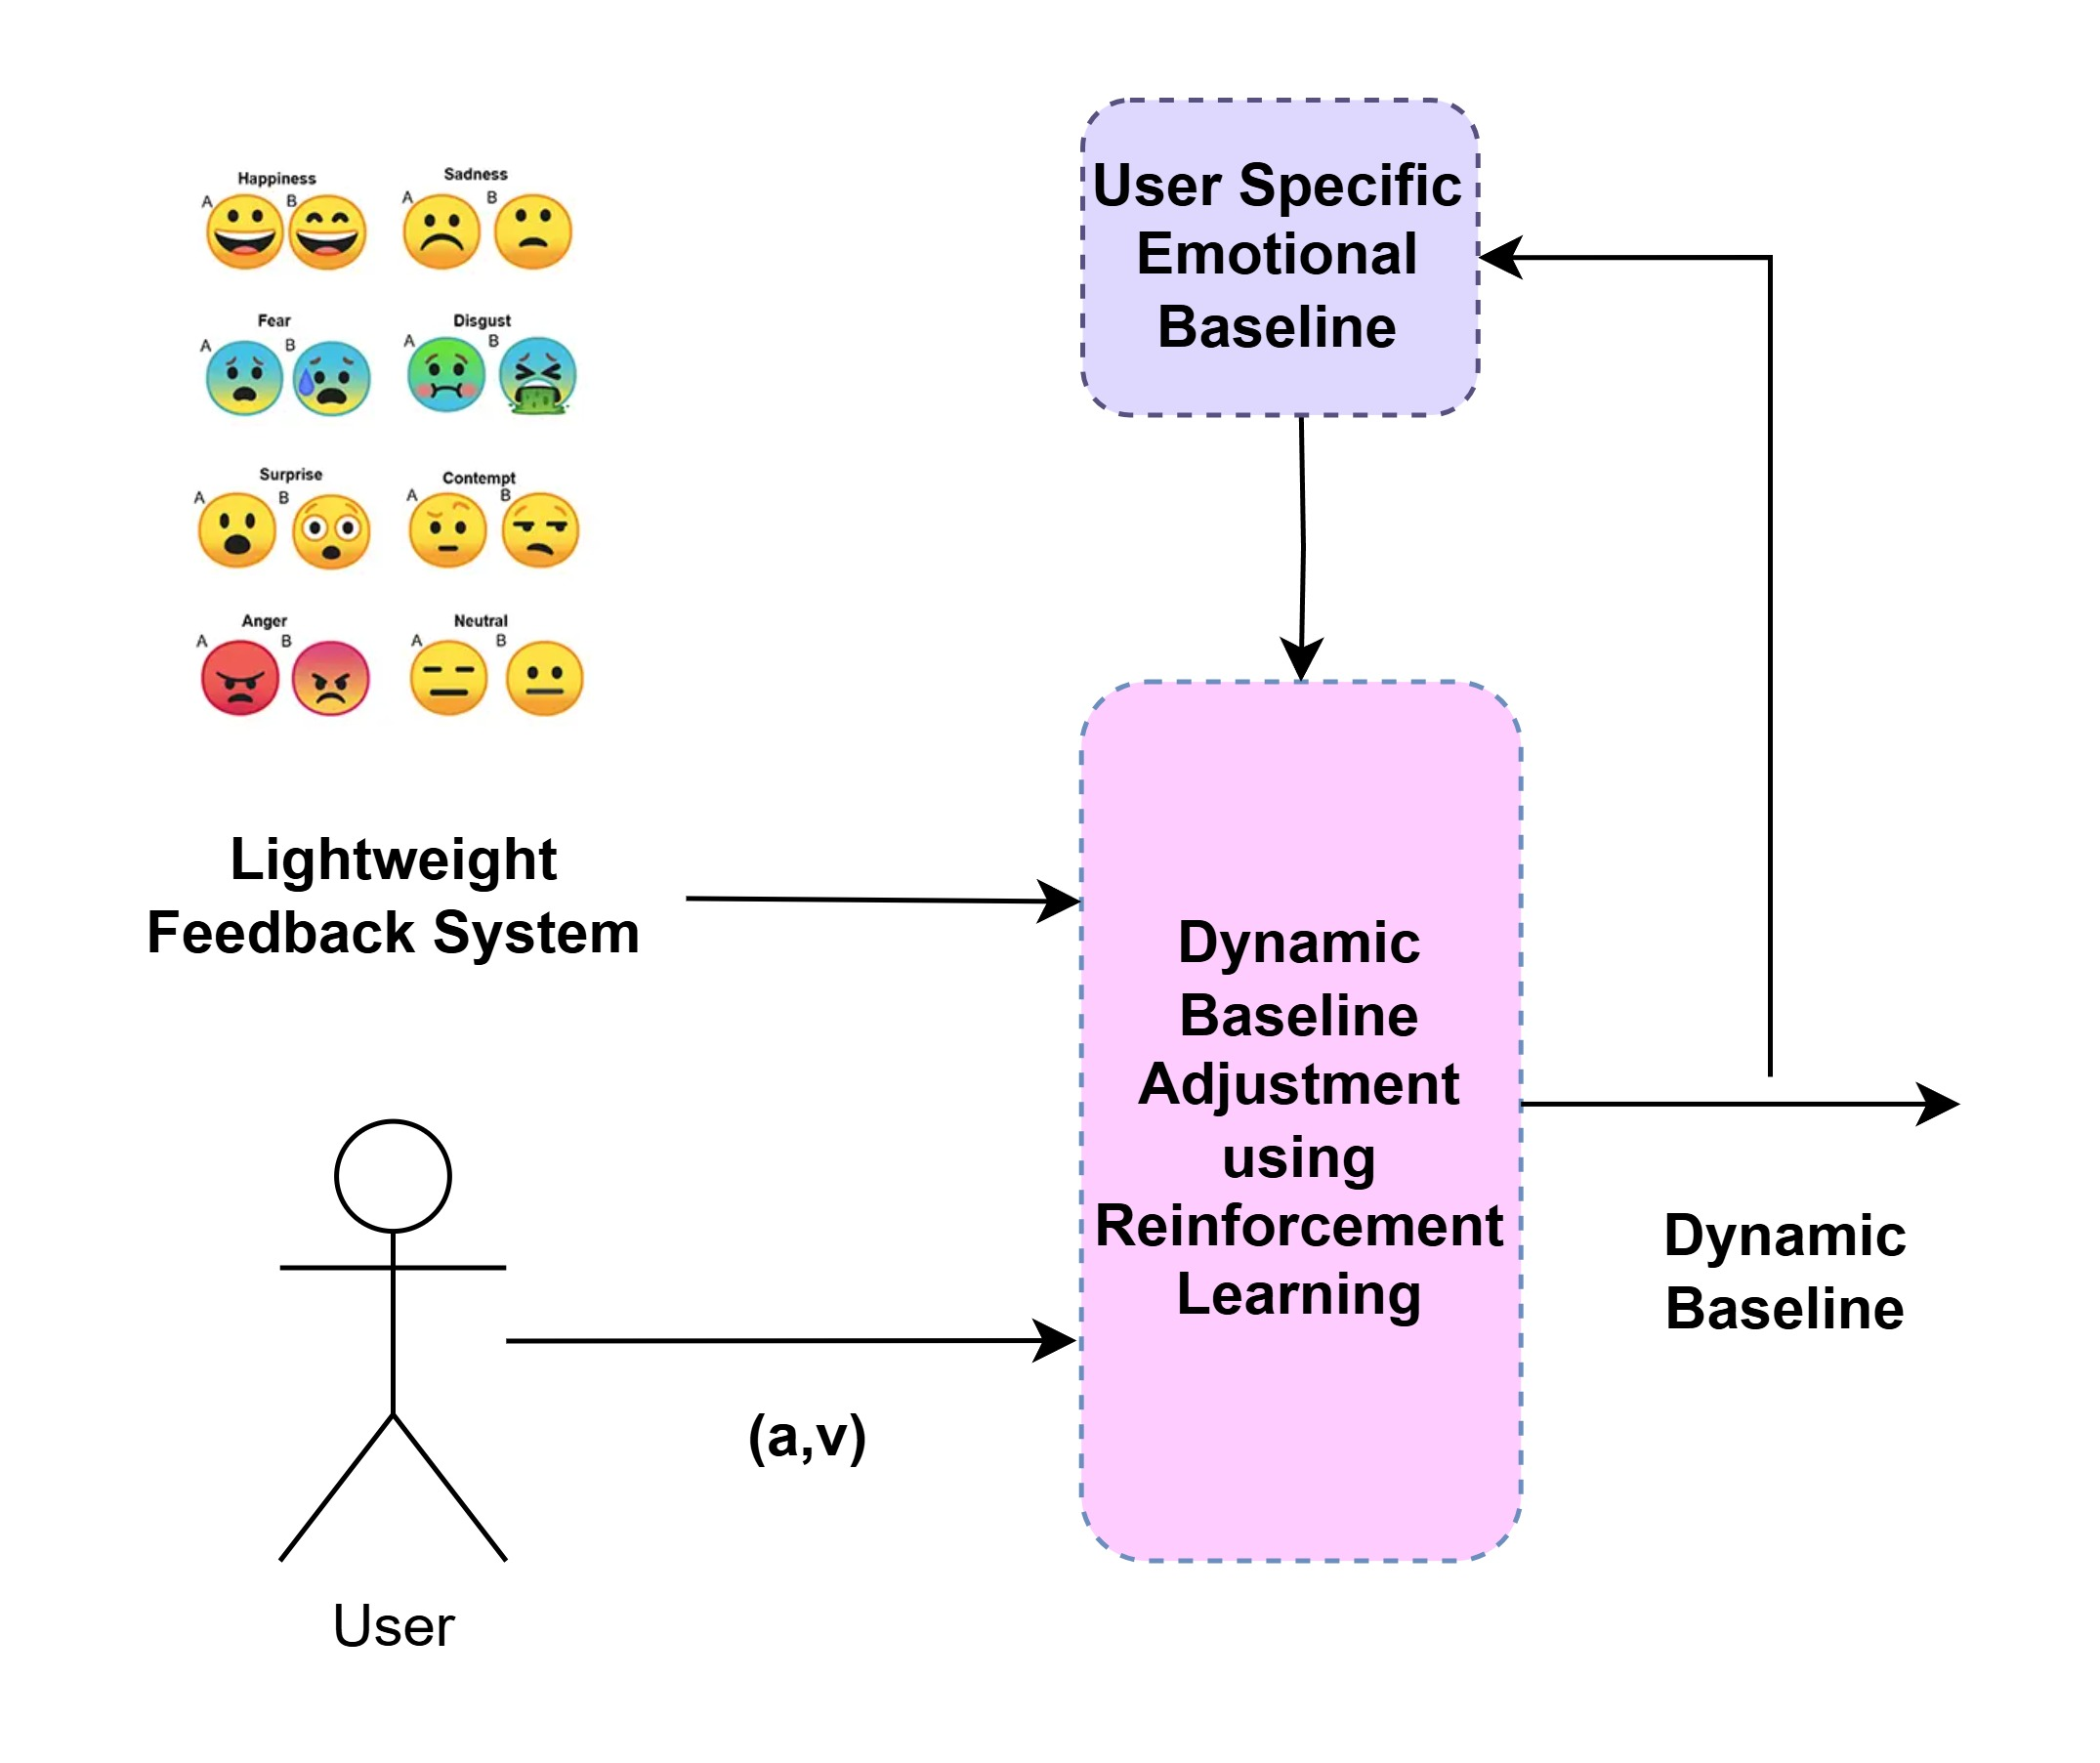
\includegraphics[width=0.7\textwidth]{img/chapter_03/Phase5.jpg}
    \captionof{figure}{Experimental flow of Phase 5}
    \label{fig:phase5}
\end{figure*}


\subsection{Relationship with Emojis and Arousal-Valence Values}

Several studies have tried to map emojis into the arousal-valence space. One important example is a study published in 2022 titled \textit{Classification of 74 facial emoji’s emotional states on the valence-arousal axes}~\cite{kutsuzawa2022classification}. This study involved 1,082 participants who rated 74 facial emojis using a nine-point scale for both valence and arousal.

The researchers used cluster analysis and one-way ANOVA to group the emojis into six main clusters. Each cluster represents a certain emotional state, going from very negative to very positive. The clusters also show how strong or intense each emotion is by using arousal values.

The table below shows the main results from the study:

\begin{table}[h]
    \centering
    \begin{tabular}{|l|c|c|c|}
        \hline
        \textbf{Cluster Label} & \textbf{N} & \textbf{Valence (SD)} & \textbf{Arousal (SD)} \\
        \hline
        Strong positive sentiment & 12 & 7.42 (0.40) & 7.19 (0.34) \\
        Moderately positive sentiment & 9 & 6.57 (0.62) & 5.98 (0.29) \\
        Neutral with positive bias & 12 & 5.49 (0.38) & 5.19 (0.29)\\
        Neutral with negative bias & 19 & 4.27 (0.38) & 4.83 (0.27) \\
        Moderately negative sentiment & 10 & 3.59 (0.37) & 5.84 (0.30)  \\
        Strong negative sentiment & 12 & 2.74 (0.40) & 6.91 (0.37)  \\
        \hline
    \end{tabular}
    \caption{Clusters of emojis and their valence-arousal values from~\cite{kutsuzawa2022classification}.}
    \label{tab:emoji_clusters}
\end{table}

This table helps us understand how different emojis can be used to reflect emotional states in both valence (positive or negative) and arousal (intensity) dimensions.

Using this idea, we built our emoji feedback mechanism. It allows users to give lightweight feedback about how they feel. This feedback is then used in the reinforcement learning stage. The overall design of this emoji feedback interface is shown in Figure~\ref{fig:emoji_feedback}.

\begin{figure}[h]
    \centering
    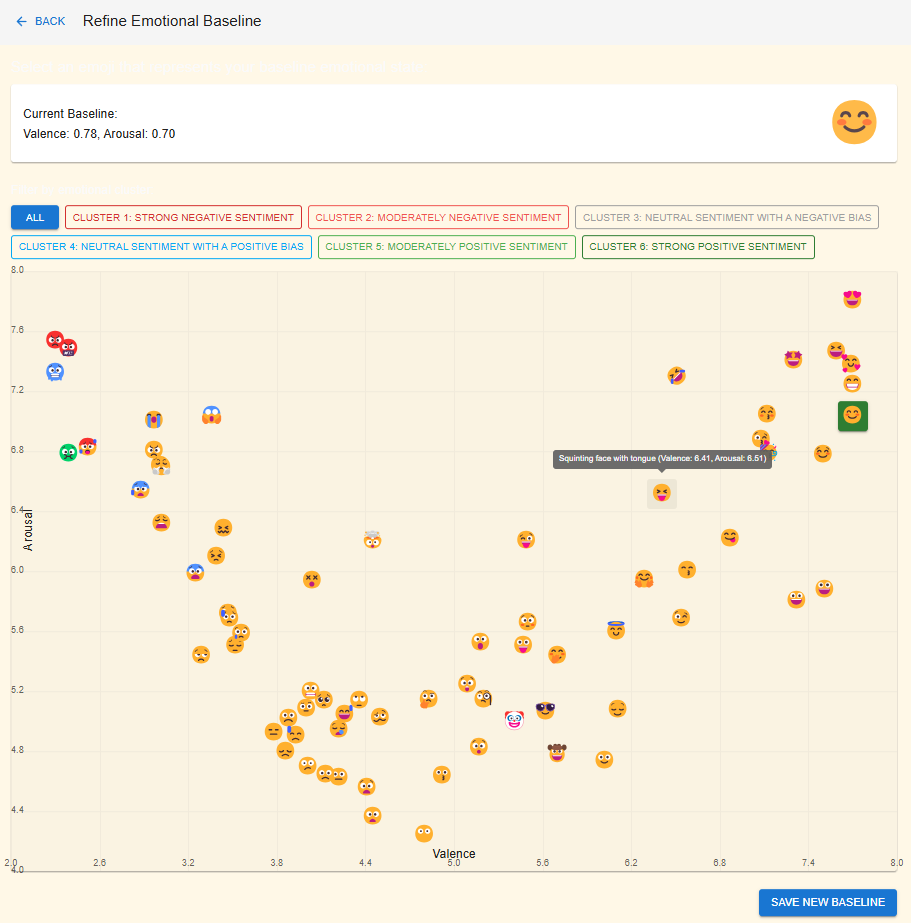
\includegraphics[width=1\textwidth]{img/chapter_03/emoji-feedback-ss.png}
    \caption{Emoji feedback interface used for lightweight user input.}
    \label{fig:emoji_feedback}
\end{figure}


